% moon phases
% Author: Andreas Kelbel
\documentclass[ngerman]{standalone}
%%%%%% Grundsätzliches 
	\usepackage[utf8]{inputenc}
	\usepackage[T1]{fontenc}
	\usepackage{lmodern}
	\usepackage{babel}
%%%%%% TikZ 
	\usepackage{tikz}
%%%%%% Schrift 
	\usepackage{cmbright}

\begin{document}
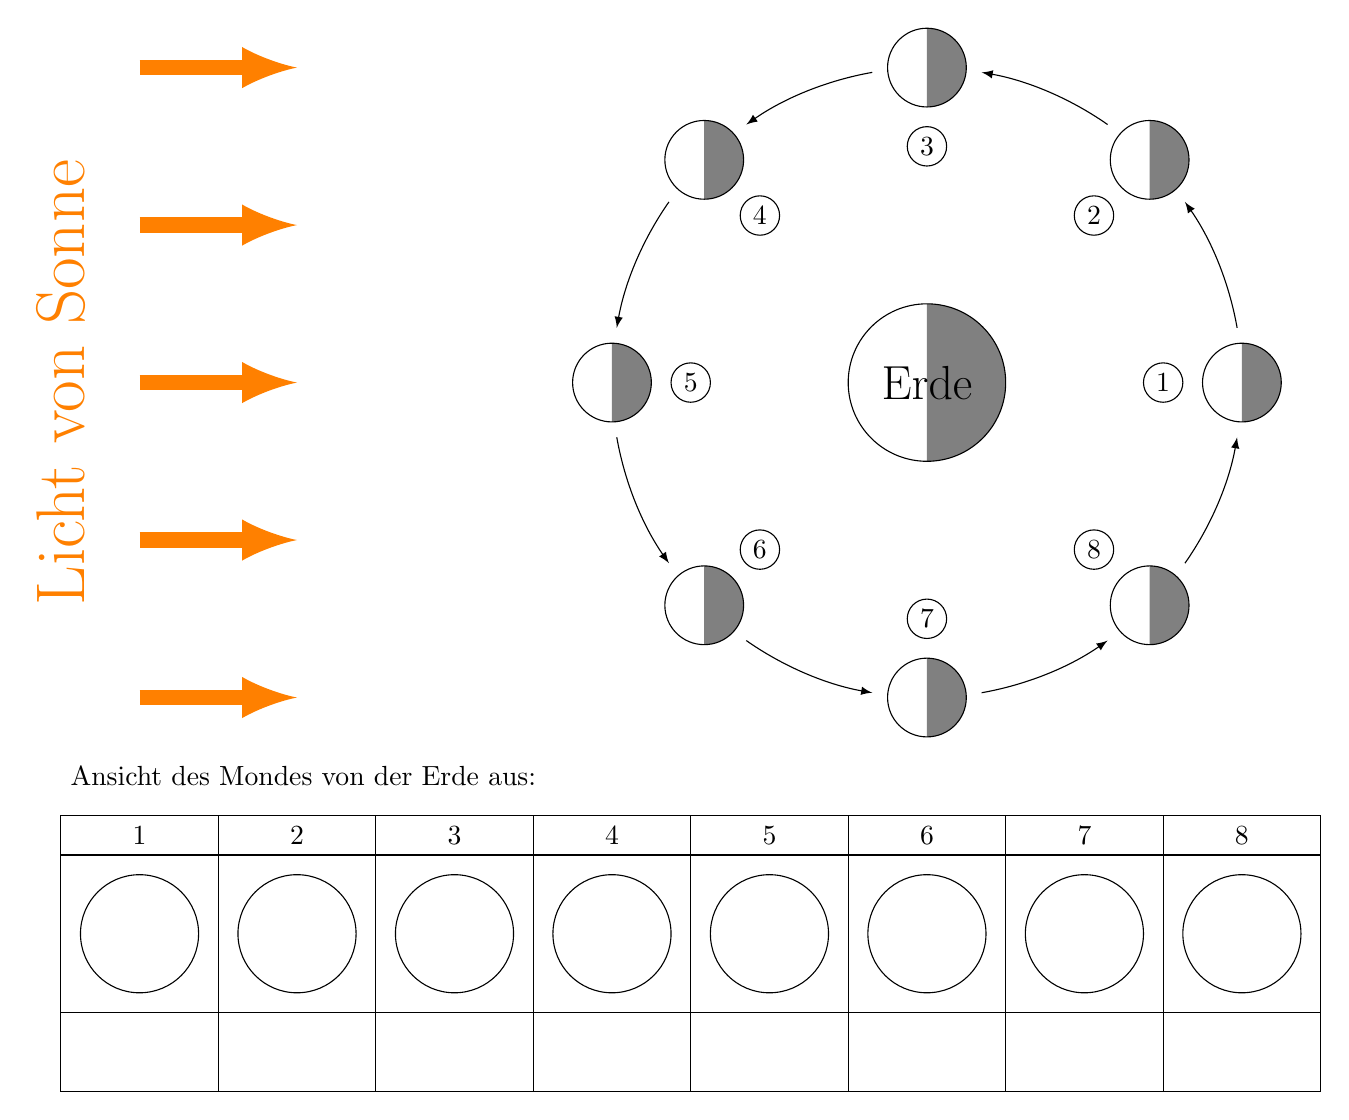
\begin{tikzpicture}
%%% Erde 
	\fill[gray] (0,0) -- (-90:1) arc(-90:90:1cm) -- (0,0) -- cycle ;
	\draw (0,0) circle (1cm) node[]{\LARGE Erde} ;
%%% Mond an verschiedenen Positionen, Pfeile	
	\foreach \i in {0,45,...,315}{
		\fill[gray] (\i:4) -- ++(-90:.5) arc(-90:90:5mm) -- (\i:4) ; 
		\draw (\i:4) circle (5mm) ; 
		\draw[-latex] (\i+10:4) arc(\i+10:\i+35:4cm) ; 
	}
%%% Beschriftung der Positionen
	\foreach \i in {1,...,8}{
		\draw (\i*45-45:3) circle (2.5mm) node[]{\i};
	}
%%% Licht von Sonne
	\foreach \i in {-4,-2,...,4}{
		\draw[-latex,line width=2mm,orange] (-10,\i) -- ++(2,0) ;
	}
	\draw[orange] (-11,0) node[rotate=90]{\Huge Licht von Sonne} ;
%%% Tabelle mit Ansicht von der Erde aus	
	\begin{scope}[xshift=-11cm,yshift=-7cm]
	\draw (0,2) node[right]{Ansicht des Mondes von der Erde aus:} ;
	\foreach \i in {1,...,8}{
		\draw (2*\i-1,0) circle (7.5mm) ;
		\draw (2*\i-2,1) rectangle ++(2,-2) ;
		\draw (2*\i-2,1) rectangle ++(2,.5) node[midway]{\i} ;
		\draw (2*\i-2,-1) rectangle ++(2,-1)  ;
	}
	\end{scope}
\end{tikzpicture}
\end{document}